\chapter{开发技术简介}

\section{技术选型与架构概述}

本章不再把项目中用到的技术逐个写成教材式介绍，而是围绕 Mini-Chat-Bar 的实际需求说明技术选型的理由。开发过程中，系统最先暴露出的并不是某个单独页面的问题，而是几类能力需要同时成立：既要完成登录、资料读取、消息保存和收藏回看等稳定的数据处理，也要支撑私聊提醒、聊天室广播、在线状态变化和 AI 增量回复这类实时交互，还要兼顾桌面端通知与托盘常驻等本地能力。单靠一种技术很难把这些事情都处理好，因此项目最终采用了前后端分层、实时通信与数据存储协同配合的方案。

如图~\ref{fig:2-1}所示，系统整体可以分为接入层、前端应用层、服务层以及数据与智能辅助层。

\begin{figure}[H]
\centering
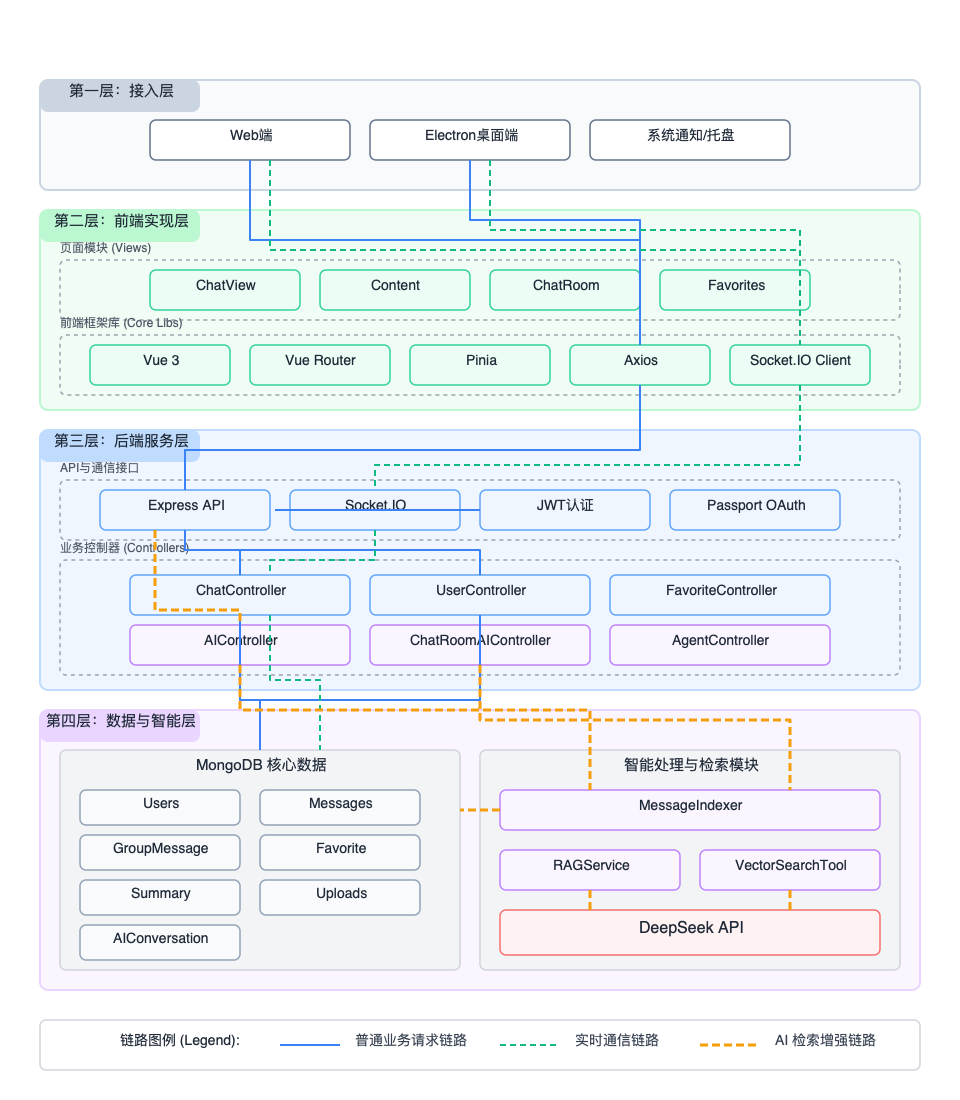
\includegraphics[width=0.76\textwidth,height=0.60\textheight,keepaspectratio]{img/图2_1.png}
\caption{系统技术架构图}
\label{fig:2-1}
\end{figure}

这样的划分不是为了把架构图画得复杂，而是因为系统中的不同任务确实需要不同链路来承担。前端主要负责界面呈现、会话切换和用户交互；服务层负责权限校验、业务处理和消息流转；数据层负责用户资料、聊天记录和收藏内容的持久化；AI 服务层则负责问答、总结和解释等增强能力。这样拆开以后，稳定的数据读写与需要即时反馈的实时交互各走合适的路径，系统结构会更清楚，后续实现和排查问题也更直接。

图~\ref{fig:2-1}并不是套用通用模板得到的，而是依据本系统已经完成的功能结构整理出来的。图中把用户管理、即时通信、聊天记录、文件管理和 AI 辅助几个部分放在同一套架构下，说明它们如何共同支撑私聊、聊天室、收藏回看和智能问答等功能。这样的表达方式也为后续章节展开总体设计、功能实现与测试验证提供了统一的基础。

\section{前端实现技术}

前端部分最明显的特点，是同一套界面中同时存在登录鉴权、会话切换、实时消息显示、聊天室详情、收藏回看和 AI 辅助等多种交互。Vue 3 在这个项目里的价值，主要体现在把这些界面拆成职责相对清楚的部分，而不是单纯为了追求新框架\cite{vueguide2026}。聊天主界面采用会话列表、消息区和详情区的三栏结构后，私聊、聊天室和收藏等功能就可以围绕各自的区域展开，界面关系也更容易理清。

状态管理由 Pinia 承担，但并没有把所有界面状态都收进全局。跨页面共享的会话状态和消息数据由状态管理统一维护，局部弹窗、搜索词和短时交互则继续放在组件内部处理。这样的划分更贴合本项目的实际需要，也减少了页面联动时的复杂度\cite{piniadocs2026}。配合 Vue Router 管理页面切换、Vite 支撑开发阶段的快速调试，再结合 Electron 补足托盘、通知和桌面常驻能力，前端部分既能保持 Web 端开发效率，也能满足桌面端展示需求。

Electron 的接入同样是围绕现有页面补能力，而不是另写一套桌面客户端。这样做保留了 Web 界面的复用效率，同时也补上了桌面常驻、消息提醒和窗口切换这些在实际使用和答辩演示中都比较直观的交互能力。

\section{后端服务与实时通信技术}

后端采用 Node.js 和 Express，并不是因为它们在 Web 项目里足够常见，而是因为这个系统从一开始就同时存在两类请求形态：一类是登录、资料读取、消息查询和收藏处理这类可以较快结束的普通请求，另一类是消息发送、在线同步和 AI 流式回复这类会持续交互的链路。把这两类请求放在同一套 JavaScript 运行环境里处理，有利于减少前后端联调时的切换成本\cite{expressdocs2026}。

本项目里 HTTP 和 Socket.IO 的分工很清楚，二者并不是互相替代。普通请求主要负责身份认证、数据读写和结果持久化，实时通道主要负责把新消息、在线状态和增量内容及时同步给在线成员。这样处理的好处很实际：稳定数据通过普通接口处理，实时变化通过长连接同步，既便于保证消息可靠落库，也便于后续定位问题\cite{socketiodocs2026}。

身份认证方面，系统采用 JWT 维护登录状态。无论用户采用邮箱密码、验证码还是第三方登录，后续访问都统一进入同一套鉴权流程。这样处理既方便权限控制，也减少了不同登录方式带来的后端分支复杂度\cite{oauthbcp2025}。

\section{数据存储与消息组织技术}

从数据组织看，虽然私聊消息、聊天室消息、收藏快照、AI 回复和讨论总结最终都会显示在聊天界面里，但它们的结构、读取方式和保存重点并不相同。私聊更强调双方关系下的历史回读，聊天室更强调按房间分页加载和多人共享，收藏更强调快照留存，AI 对话和总结则需要保留上下文信息。基于这种差异，系统采用 MongoDB 存放主要业务数据\cite{mongodbdocs2026}。

结合实际访问路径，系统把用户、聊天室、消息、收藏和 AI 相关数据分别组织，历史消息重点围绕会话或房间读取，收藏内容则便于后续筛选和回看。文件资源与消息记录分开保存，只在消息中保留必要的展示与定位信息。这样的设计不追求形式上的复杂，而是服务于当前项目里最常见的读取与回看需求。

索引设置同样跟着读取方式走。常用查询集中在最近会话、按时间回读历史消息、按房间查看讨论和按用户查看收藏等场景，因此数据库优化也围绕这些高频路径展开。对本科毕业设计的系统规模来说，这样的组织方式已经足够支撑消息分页、历史检索和收藏沉淀等主要功能。

\section{AI辅助技术}

本系统中的 AI 不是附加在聊天界面旁边的演示功能，而是直接参与技术讨论过程。侧边栏 AI 助手更适合单人连续追问，也可以用于对选中的术语、报错信息或代码片段做解释；聊天室内的 AI 问答和阶段总结则面向多人协作，回答结果能够继续留在房间里被所有成员查看和引用。

如果只把用户最后输入的一句话直接交给模型，回答很容易脱离前文。为了解决这个问题，项目在聊天室问答链路中加入了消息索引与检索增强。问答发起前，系统会先从当前房间的历史消息中召回相关讨论，再把这些上下文与用户问题一并提交给模型。这样得到的回答更贴近房间里已经形成的讨论脉络，而不是把每次提问都当作一条孤立的新问题。

考虑到 AI 回复明显慢于普通接口，系统采用流式输出方式逐步返回内容，让提问者和房间成员都能及时看到回答进展。这种做法虽然没有改变模型本身的响应速度，但能明显改善交互体验。

当前实现还保留了一个务实的降级方案：当外部向量或 embedding 服务不可用时，系统仍可退回本地检索方式，先保证开发环境和答辩环境能够跑通整条链路。结合历史消息回读、聊天室总结与 AI 回复持久化功能，AI 在本系统里的角色更接近“利用已有讨论提供辅助”，而不是替代用户完成全部交流。

为了更清楚地说明大语言模型与系统内业务数据的结合方式，图~\ref{fig:2-2}给出了本系统 RAG（检索增强生成）的核心流程。

\begin{figure}[H]
\centering
\thesisfigwide{img/图2_2.png}
\caption{RAG 检索增强生成原理图}
\label{fig:2-2}
\end{figure}

如图~\ref{fig:2-2}所示，整个智能问答可以概括为“先组织历史上下文，再生成回答”两个环节。用户发送问题后，系统先整理与当前话题相关的历史消息，再将其与当前提问一并提交给模型；模型返回结果后，系统按普通消息或流式消息的形式展示出来。这套设计的重点不在于堆叠更多 AI 术语，而在于让回答尽量贴近当前聊天室已经形成的讨论上下文。
